\section{Motivation}

Despite the increasing pervasiveness of mobile devices, as noted by \citet{socialTV}, there is a surprisingly limited number of options for mobile users to access live streaming television. Tablet computers in particular open up diverse and interesting interactivity questions -- could exploiting physical interaction hold viewers attention, even during adverts they may otherwise have ignored? Furthermore, could the disparity in the number of viewers per viewing device between traditional televisions and mobile devices be constructively exploited to provide granularly targeted adverts?

In this section, we will first introduce the customer of this project, \textit{Inqb8r}, and explain their interest in the area of TV streaming on tablet computers. We'll examine the functionality of tablet computers and question the benefits that the pervasiveness, mobility and interactivity of them provide. We will then consider how suitable current television formats would be for tablet computers, and following this, consider how this could open up opportunities for new methods of advertising by utilising interactivity and granular targeting. We will summarise by explaining how these insights could improve viewer attentiveness to adverts and the relative impacts on the advertisers and users of such a platform.

\subsection{Interest by Inqb8r}
	\label{sec:motivation_inqb8r}
	
	This project has been the result of a project proposal (Appendix~\ref{sec:inqb8r_proposal}) by \textit{Inqb8r}\footnote{Inqb8r's website -- \footurl{http://inqb8r.tv}} for a TV service targeted at tablet computers that would make use of complimentary services, such as interactive overlays and supplementary statistics. Inqb8r is a UK based business which provides a platform for content owners and advertisers to expose their products and services to university students.

	Inqb8r are responsible for the development of Project4\footnote{Project4's website -- \footurl{http://www.project4.tv}} (Figure~\ref{fig:project4}), a TV streaming service targeted towards students on Janet\footnote{Janet is a private network for education and research -- \footurl{https://www.ja.net/}}. Students are able to access the Project4 website in order to stream Channel~4, E4, More4, Film4 and 4Music, as well as it's own TV channel, studentTV. Project4 replace adverts broadcast by Channel~4 with adverts targeted specifically towards students.
	
	\begin{figure}[htb]
		\centering
			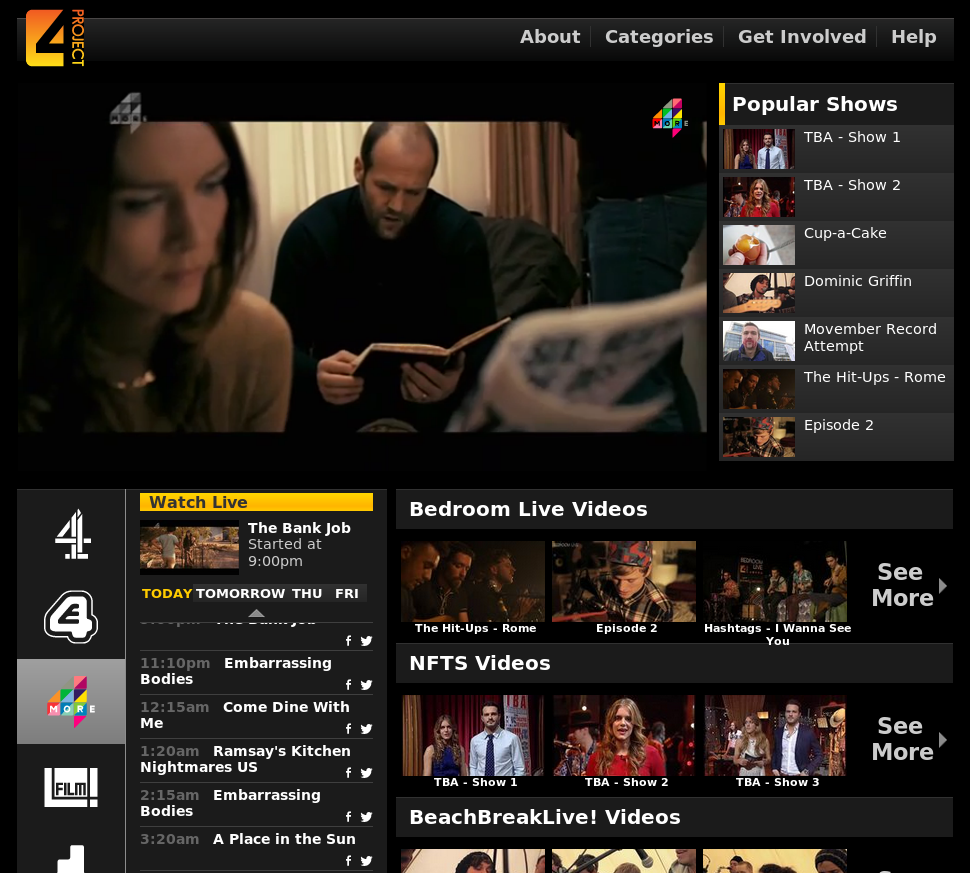
\includegraphics[width=0.5\textwidth]{images/project4.png}
		\caption{Project4 -- a student-oriented web-based TV service, which offers Channel~4 channels with adverts replaced with student-focused adverts.}
		\label{fig:project4}
	\end{figure}

	Inqb8r are interested in expanding the reach of Project4 by the creation of an application to watch TV on tablet computers. At present most of their users access the service via a web browser. This is in part due to their use of a Flash based player which is not compatible with many mobile devices, including iPads and other Apple devices. Modern technologies -- in particular, HTML5 -- allows video streaming in a web browser on these devices.

	Inqb8r expressed strong interest in researching how the touch displays and accelerometers of tablet computers may be used in providing interactive TV. One suggestion was to investigate the use of interactive overlays -- additional information displayed on top of a video stream, such as links to supplementary information, live polls and chats. They expressed interest in understanding how such overlays would affect how viewers watch TV.
	
	%utilisation of new HTML5 technologies to open up their service to a wider audience. Furthermore as their software utilises an interactive overlay for basic control they are interested to see how interaction centric platforms such as iPads can be leveraged to provide greater viewer interest. They are particularly keen to see if integrating traditional second screen technologies directly into the viewing medium has an impact on usability and enjoyability. 

\subsection{Pervasiveness of tablet computers}
	% Why would tablet computers be an interesting area to research?

	The popularity of tablet computers has been increasing rapidly. In 2012, \citet{pewResearch} showed that 25\% of Americans now own tablet devices and \citet{viacom} states that 15\% of full length television shows are now watched on tablet devices. Statistics collected by the TabLens service\footnote{The Tablens Service -- \footurl{http://www.comscore.com/Products/Audience_Analytics/TabLens}} support this, showing that most tablet owners use their tablet to watch video\footnote{Comscore -- Majority of Tablet Users Watch Video on their Device, 1 in Every 4 Viewers Pay to Watch (June 2012) -- \footurl{http://www.comscore.com/Insights/Press_Releases/2012/6/Majority_of_Tablet_Users_Watch_Video_on_their_Device}}. Furthermore, statistics\footnote{International Data Corporation (IDC) Raises Tablet Forecast for 2012 and Beyond As iOS Picks Up Steam, Android Gains Traction, and Windows Finally Enters the Market -- \footurl{http://www.idc.com/getdoc.jsp?containerId=prUS23833612}} from IDC (see Figure~\ref{fig:tablet_market_share}) show that the Apple iPad holds the largest market segment and their predictions for 2016 suggest that Apple will maintain a strong majority if current trends do not change.

	\begin{figure}[h]
		\centering
			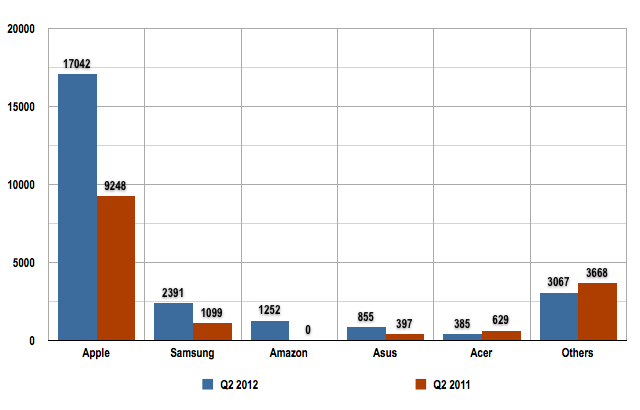
\includegraphics[width=0.6\textwidth]{images/idcTabletMarketShare.png}
		\caption[Caption for LOF]{Tablet Market Share (from reghardware.com\footnotemark, data source: IDC)}
		\label{fig:tablet_market_share}
	\end{figure}
	\footnotetext{Tablet market share -- \footurl{http://www.reghardware.com/2012/08/02/apple_leads_tablet_market_but_rival_shows_greater_growth/}}

	The mobility of tablet computers allows people to consume content from almost anywhere. Close to 40\% of Americans use their smartphones or tablets to watch TV at least once a day \citep{state-of-media}. \citet{google-tablets} presents the wide range of tablet usage locations, including at the home, in the car, in a public place, at the gym, in the classroom and whilst commuting. The study indicated interviewees who used the tablet for video consumption liked the tablets bigger form factor compared to their phone. Participants also indicated that they had migrated some activities away from their laptops and smartphones to their tablet. It is suggested that the activities users migrate tend to be leisurely, and reflect the users perception of the device being ``fun''. These factors indiciate a growing pervasiveness of tablet computers, as users switch to tablets for media consumption from other, less suitable, devices.

\subsection{Evolution of television viewing}
	\label{sec:evolution_of_TV}
	
	Since the invention of television, shows have been broadcast sequentially in the form of \textit{channels}. The number of TV channels is restricted by the availability of radio-wave frequencies, however, digital broadcasting allows multiple channels to be encoded into a radio band \citep{DTVTransmission}. This has led to a dramatic increase in the number of TV channels and has allowed broadcasters to expand their number of channels -- for example, Channel~4 (originally just one channel) now broadcasts six channels\footnote{Channel 4 Channels: Channel 4, E4, More4, 4Music, Film4, 4seven}. Broadcasters can now provide more content at any one time and improve their reach by targeting multiple groups of people.

	However, this large choice of channels makes it difficult and frustrating for an individual to find a show to watch \citep{cisco10Reasons}. TV listings are two-dimensional: an individual must search for a particular time under a particular channel in order to find a programme on at that time. This problem may be partly mitigated by Electronic Programme Guides (EPG) -- TV listings that are available electronically on digital TV receivers. An EPG may allow an individual to view what programmes are starting soon and even restrict what programmes are shown based on a viewer's interests \citep{informationOverload}. While this reduces the channels an individual has to search through, viewers are still limited to the choice of what is on at that particular time.

	This difficulty in finding a suitable programme leads to longer time spent switching between channels. During this time (the transit time), viewers potentially miss adverts. Advertisers therefore must pay for more advert spots to counter this. Even if the advertisers pay for an advert spot longer than the average transit time, having not seen the full advert, viewers who arrive late may not receive the full impact of the advert. Research has shown that the number of opportunities to see (OTS) an advert affects how effective that advert is \citep{OTS}. \citeauthor{OTS} discusses an optimum OTS of three in order to achieve maximum return on investment. If we assume that channel switching would not be a problem and adverts would subsequently not be missed, an advertiser would need to purchase less advert spots in order to achieve this OTS, maximizing its return on investment.

	%Modern on-demand services, such as BBC iPlayer and 4oD, allow individuals to view what they want at any time. The choice of programmes may be huge, however, and may not be suitable for a user of a mobile device where searching is a problem due to... and may be frustrating

	The increased number of channels and range of methods of viewing TV has led to less viewers concentrated in any one area. This fragmentation of the TV-viewing market, has been observed by \citet{audienceFragmentation} and \citet{informationOverload}. Advertisers are able to target specific markets by advertising on channels that fill a niche, such that the music channel 4Music. Understanding the market of a niche channel is far easier than predicting the average viewership of the channel. However, in order to achieve the reach of a less fragmented market, spots on a large number of channels must be purchased \citep{addressableAdvertisingOnDigitalTV}.

	%Furthermore, \citet{o2004improving} discusses
	%EPG navigation by providing intelligent guides such as that in 
	%reducing the transit path such as in \citet{personalisedEPG}

	%While modern systems allow EPG data to be displayed and searched on the TV the fact that TV is live means that by the time a user has located a desirable show it may already have started. This is somewhat resolved by time-shifted channels which are simply rebroadcasts of other channels at a later time such as E4+1. Some services have also started offering 2 hour shifted channels but these still require a user to be present and ready at the exact time of broadcast. If users are more able to move to their next optimal channel, while minimising the transit time, this will mean they see a greater number of relevant adverts in a given usage period as they would be on a channel showing appealing content for a greater percentage of their time, hence if advertisers target their adverts to the shows well, then improving this situation could significantly improving the OTS values of relevant adverts.

	
\subsection{Beyond traditional advertising}
	\label{sec:beyond_traditional_advertising}

	Advertisers pay for advert spots when they believe their target audience will be watching, but it is unlikely that all viewers will be interested in the adverts. The user experience of any viewers who are not interested in the advert is negatively impacted in these situations. Some services, such as YouTube, have added the ability to skip adverts (see Figure~\ref{fig:skip_youtube_ad}). This improves their overall user experience as viewers that find an advert annoying or offensive have the ability to skip it. Furthermore other systems, such as Facebook, allow users to close adverts after explaining why (see Figure~\ref{fig:close_facebook_ad}). This feedback can help prevent inappropriate adverts and allow advertisers to improve their future advertising campaigns. 

	\begin{figure}[!h]
		\centering
		\begin{subfigure}[h]{0.6\textwidth}
			\centering
			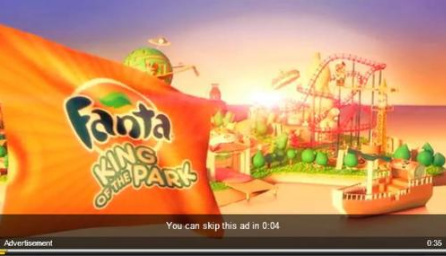
\includegraphics[width=\textwidth]{images/youtube_ad.png}
			\caption{YouTube allows adverts to be skipped after a designated duration.}
			\label{fig:skip_youtube_ad}
		\end{subfigure}
		\begin{subfigure}[h]{0.39\textwidth}
			\centering
			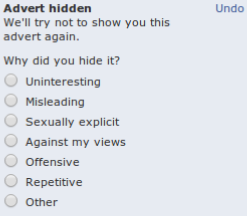
\includegraphics[width=\textwidth]{images/facebook_ads.png}
			\caption{Facebook asks why an individual closes an advert.}
			\label{fig:close_facebook_ad}
		\end{subfigure}
		\caption{Approaches to allowing individuals to close or skip adverts.}
		\label{fig:advert_skipping}
	\end{figure}

	We hypothesise that users would be more likely to enjoy adverts if they were relevant to their interests. With this assumption, we can infer that personally recommended adverts targeted to each user would improve user interest, thus improving the user experience. This could provide advertisers with greater conversions per impression by maximising the likelihood that a viewer will be interested in their product. Furthermore, allowing users to blacklist adverts should improve the user experience by giving users the opportunity to control which adverts they see and, if they provide a reason for their disapproval, provide feedback to advertisers such that they can improve future adverts.

	We hypothesise that if a user is less engaged by an advert then they may ignore it or be easily distracted. Second screen applications, such as Shazam\footnote{Research Proves Shazam-Enabled TV Advertising Extends Engagement and Improves Effectiveness -- \footurl{http://www.businesswire.com/news/home/20121118005054/en/Research-Proves-Shazam-Enabled-TV-Advertising-Extends-Engagement}}, allow users to perform related tasks such as tagging the adverts which they see. This has been shown to increase brand recall, but involves performing a supplementary task, drawing attention from the advert. Providing interactivity \textit{within} the adverts would reduce loss of attention an allow advertisers to provide useful or fun interactive content to reinforce the advert.

	By keeping the user focussed on the advert, even if they do not pay direct attention to the content, interaction provides another chance for users to remember the advert. It provides greater benefit in repeated adverts, as users may interact with the advert again if it is entertaining or useful. For example, a trailer for an upcoming film may use location data to show the closest showings. When the user first sees the advert they may not be looking for a film, but may at a later point. Interaction also gives opportunity to integrate with social networks. For example, the action of liking something on Facebook allow users to save information on their personal profiles for later reference, improving brand recall.

\subsection{Individual targeting}
	\citet{socialTVPaper} argues that television is defined by the content that is viewed, not the device it is viewed on. While a traditional TV is often viewed by many individuals at once, such as a family, tablet computers are typically used by a single person. This means that adverts can be targeted individually. It is argued that social networking has a direct impact on what is broadcast -- users can provide feedback to broadcasters on, for example, Twitter. \citeauthor{socialTVPaper} further suggests that encouraging social participation in advertising would further allow users to control what they see and provide rich feedback to the advertisers. This effect has been studied in \citep{socialTV}.
